\section{Test Results}\label{sec:Test}
In this section, we verify that simualations give useful results, and evaluate to what extend \tech improve traffic flow and reduce fuel consumption.

\subsection{Verification of the Simulator}
It is imporant to verify that the results obtained from the simulator actually matches the real-world observations.
We compare the results from the simulator with GPS trajectories collected in the project "Spar P\aa Farten".
If the results are similar, we may deduce that the simulator provides usable results.
We compare the simulator with the GPS data on three fronts: 
\begin{enumerate*}
\item Comparison based on a metric based on average speed, number of stops and waiting time
\item Comparison of the travel distance 
\item Comparison of the driving speed
\end{enumerate*}

We only look at data from the main road of Hobrovej in the northern direction, only use GPS trajectories between 10 am and 2 pm on weekdays, and use a spawning rate of $0.8$ vehicle per second.%TODO: Check
Tests show that this give comparable data.

\subsubsection{Validation Metric}
The validation metric is based on three key measurements: speed, waiting time and number of stops. 
Waiting time is the difference between the travel time and free flow time, which is how long it will take to drive the same distance driving at the speed limit and never stopping.
The free flow time is $93.?s$. %TODO: What was it?
We say a vehicle has stop when its speed drops below $10km/s$, and say that it move again when it drives faster than $15km/h$.
The average value for all vehicles on the main road of Hobrovej togeather with the population standard deviation (STDEV) can be seen in Table~\ref{table.valMetric}.
The differences between average speed and average waiting time are minimal indicating that SUMO simulates these factors satisfactory.
The number of stops varies more, and the deviation is significant. 
The vehicles do, however, not stop very often, which can make the values inaccurate. 

\begin{table}
\centering
\begin{tabular}{|l|c|c|c|c|}\hline
 						&  \multicolumn{2}{c|}{SUMO} & \multicolumn{2}{c|}{GPS} \\\hline
 						& Value & STDEV & Value & STDEV \\\hline
Avg. speed ($km/h$) 	& 37.45 & 7.86 	& 36.11 & 6.32 \\\hline
Avg. waiting time ($s$) & 66.90 & 33.97 & 63.90 & 28.15 \\\hline
Avg. number of stops 	& 1.91 	& 0.66 	& 1.60 	& 0.92 \\\hline
\end{tabular}
\caption{Validation metric}\label{table.valMetric}
\end{table}

\subsubsection{Travel Distance}
Travel distance of the real data is plotted in Figure~\ref{fig:TestResults:realDistance} as a function over time. 
We see that the curves flatens at about 300 $m$, 600 $m$, 900 $m$ and 1200 $m$, indicating that the vehicles are stationary at these points.
This corresponds well with the dimensions of Hobrovej and match the four regulated traffic lights.
\begin{figure}[htb]
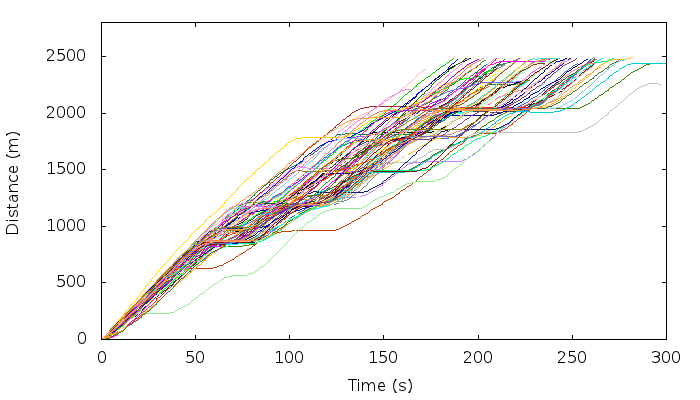
\includegraphics[width=0.45\textwidth]{../images/Real/RealDistance.png}
\caption{Travel distance for real GPS trajectories}
\label{fig:TestResults:realDistance}
\end{figure}

Figure~\ref{fig:TestResults:distance0} also plots the travel distance as a function over time, only for the results of the simulator.
We see that the simulation resembles the real-world results, however, the simulated vehicles tend to hold longer at the traffic lights. 
This is because the phases of traffic lights of the simulation are too different compared to real traffic lights. 
Besides that, the acceleration profiles look similar, and the map has the correct dimensions.

\begin{figure}[htb]
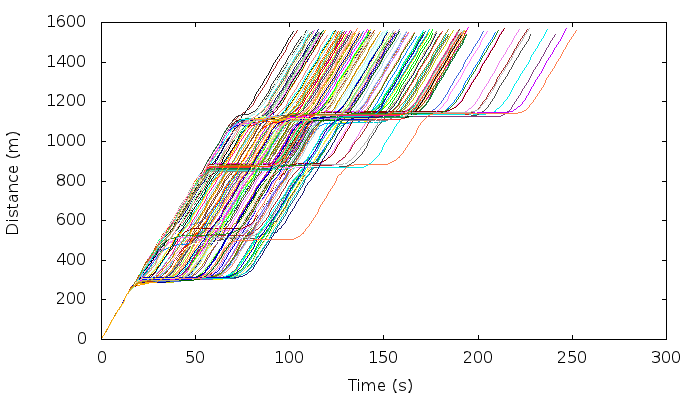
\includegraphics[width=0.45\textwidth]{../images/tp0c0_8/distanceUncontrolled0.png}
\caption{Travel distance for simulated data without \tech}
\label{fig:TestResults:distance0}
\end{figure}

\subsubsection{Driving Speed}
The driving speed as a function over time for the GPS trajectories is plotted in Figure~\ref{fig:TestResults:RealSpeed}.
In order to read the data, only random 20 trajectories have been plotted in this graph.
First of all, we see that most drivers drive at around $50 km/h$, and some drives above the speed limit of $60 km/h$. 
We also see that many drop to around $0 km/h$ and that some are able to avoid a full stop.

\begin{figure}[htb]
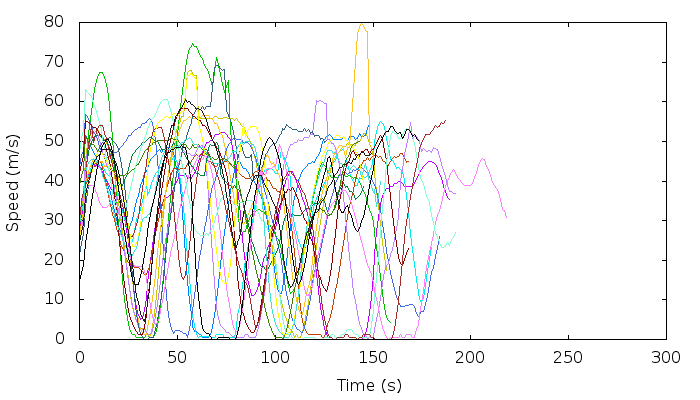
\includegraphics[width=0.45\textwidth]{../images/Real/RealSpeed.png}
\caption{Speed for real GPS trajectories}
\label{fig:TestResults:RealSpeed}
\end{figure}

Plots of the driving speed for the simulated vehicles can be seen in Figure~\ref{fig:TestResults:speed0} as a function over time.
The behaviour of these simulated vehicles are much different from the real drivers.
The simulated drivers almost always either accelerate to the maximum speed or decelerate to $0 km/h$. 
A few decelerates to $40 km/h$, but that is most likely because the traffic light turns green just before they arrive.
No one breaks the speed limit.
The simulated vehicles therefore have a much more aggresive driving behaviour than what we see in the real world data.
This will also mean that they use more fuel than a real driver would use.
However, we see that the metric values for the real and simulated data are not that different.

\begin{figure}[htb]
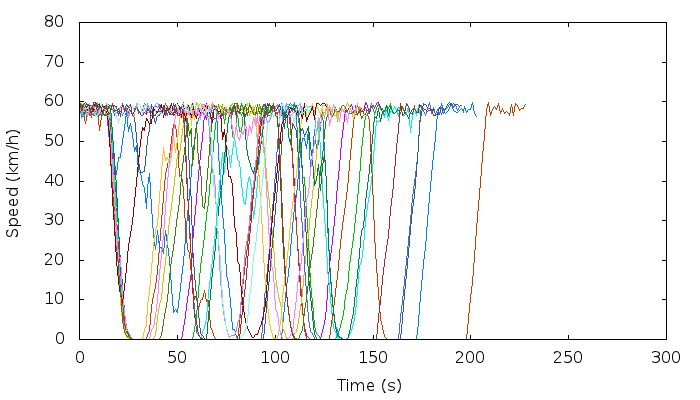
\includegraphics[width=0.45\textwidth]{../images/tp0c0_8/speedUncontrolled0.png}
\caption{Speed for simulated data without \tech}
\label{fig:TestResults:speed0}
\end{figure}

\begin{table}
\centering%TODO: Update
\begin{tabular}{|l|l|cc|cc|}\hline
Percent using 			& With/w.o. & \multicolumn{2}{c|}{Fuel} 	& \multicolumn{2}{c|}{Time}\\
\tech					&\tech		& $ml$		& Diff.			&	$s$	& Diff.\\\hline
\multirow{1}{*}{0\%}	& Without	&	128.4	&	0\%			&	157 & 0\%		\\\hline
\multirow{2}{*}{10\%}	& With 		&	93.5	&	27.2\%		&	151 & 3.8\%		\\
						& Without 	&	127.5	&	0.7\%		&	151 & 3.8\%		\\\hline
\multirow{2}{*}{50\%}	& With		&	89.0	&	30,7\%		&	144 & 8.3\%		\\
						& Without	&	122.2	&	4.8\%		&	139 & 11.5\%		\\\hline
\multirow{1}{*}{100\%}	& With		&	86.5	&	32.6\%		&	125 & 20.4\%	\\\hline
\end{tabular}
\caption{Average values with out sensors. Diff. is the difference compared to 0 \% using \tech}
\label{tb:TestResults:total}
\end{table}

\subsection{Fuel Consumption}
Reducing the fuel consumption at least for the vehicles using the system is one of the objectives.
No real data on the fuel consumption is aviable to us, and we therefore only compare the simulation with itself. 

Figure~\ref{fig:TestResults:fuelTotal} plots the fuel consumption for all vehicles in the network for two different simulations: one where no vehicles use \tech (blue) and one where all vehicles are using \tech (green).
The amount of vehicles are the same in both simulations, and they drive the same routes with the same departure times. 
The only difference is whether they use \tech or not.

The average fuel consumption when all vehicles use \tech is about $90 ml$ and about $130 ml$ when no one use \tech.
We therefore see a significant overall reduction in fuel consumption on about 20 \% in this setting if \tech is used by everybody.
Looking at just the selected route through the network, we see the same tendency (see Figure~\ref{fig:TestResults:fuelRoute}). 
The average fuel consumption with \tech is about $87 ml$ and about $126 ml$ without, resulting in a reduction at 31 \%.
%TODO: Consider using 10% in stead of 100% in the two figures below.
\begin{figure}[htb]
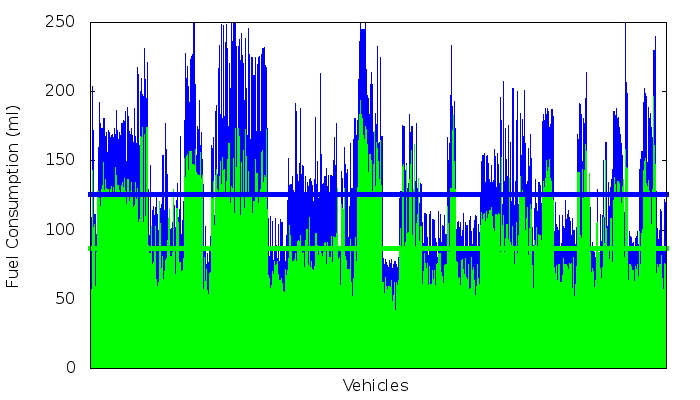
\includegraphics[width=0.45\textwidth]{../images/tp0c0_8/fuelTotal.png}
\caption{Fuel consumption for all vehicles in the network. Blue: 100\% using \tech, green: 0\% using \tech}
\label{fig:TestResults:fuelTotal}
\end{figure}

\begin{figure}[htb]
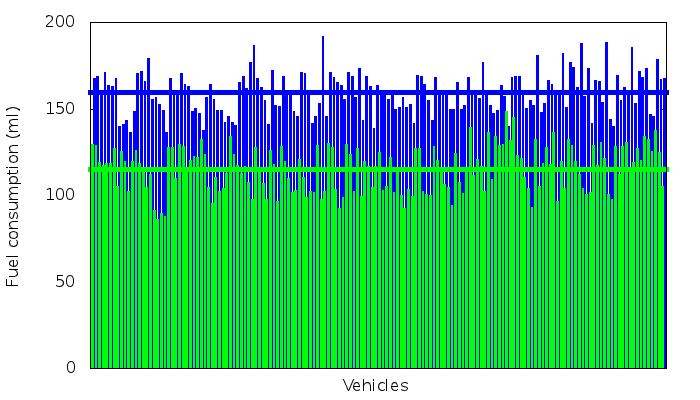
\includegraphics[width=0.45\textwidth]{../images/tp0c0_8/fuelRoute.png}
\caption{Fuel consumption for all vehicles on the selected route}
\label{fig:TestResults:fuelRoute}
\end{figure}

It is, however, more interesting to investigate the influence \tech has when only a few drivers use it.
Figure~\ref{fig:TestResults:combinedFuel} shows the average fuel consumption for four different penetration rates (0 \%, 10 \%, 50 \% and 100 \%) on the main route.
The blue columns show the average fuel consumption for those not using \tech, and the green columns show the average fuel consumption for those using \tech.
The left- and rightmost columns hence show the same average levels as in Figure~\ref{fig:TestResults:fuelRoute}.
When \tech is used in 10 \% of the vehicles, we see a small decrease in fuel consumption for those not using it, and a significant reduction for those using \tech.
The reduction is about 29 \% (reduced to $ml$).
When the penetration rate increases to 50 \%, we again see that the fuel consumption decreases slightly for those not using \tech, but see that it increases slightly for those using it.
This is most likely because vehicles start platooning (driving in groups), where vehicles using \tech force other vehicles to drive slower and the recommended speed may match the traffic lights less when the vehicles huddle together.

\begin{figure}[htb]
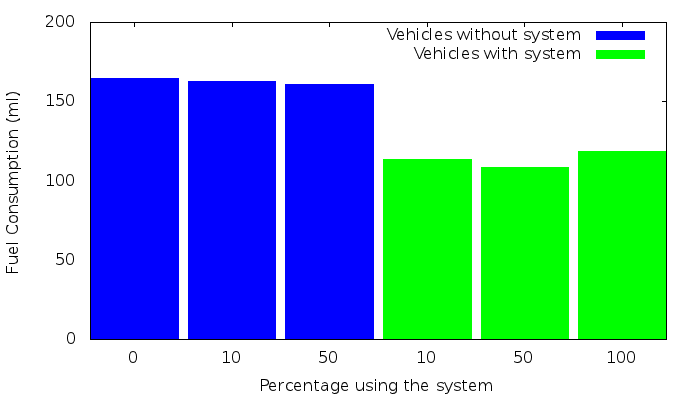
\includegraphics[width=0.45\textwidth]{../images/tp0c1_0/combinedFuel.png}
\caption{Fuel consumption for different penetration rates on the main route}
\label{fig:TestResults:combinedFuel}
\end{figure}

We see this fuel reduction because the vehicles accelerate less rapidly. 
Figure~\ref{fig:TestResults:distance100} shows the travel distance as a function over time when all vehicles use \tech, and Figure~\ref{fig:TestResults:speed100} plots the driving speed as a function over time.
We see that the curves are much more smooth than those in Figure~\ref{fig:TestResults:distance0} and~\ref{fig:TestResults:speed0}, because they avoid stopping, and hence has to accelerate less.
Some vehicles still have to stop, partly because it is impossible to drive the distance between the traffic lights in the amount of time left before it turns green, and partly because there are other vehicles blocking their path.

We can therefore conclude that in the tested use case, we see a significate reduction in fuel consumption even when it is only implemented in a small subset of the vehicles. 
Moreover, vehicles using \tech does not have a negative influence the other fuel consumption of the vehicles.
\begin{figure}[htb]
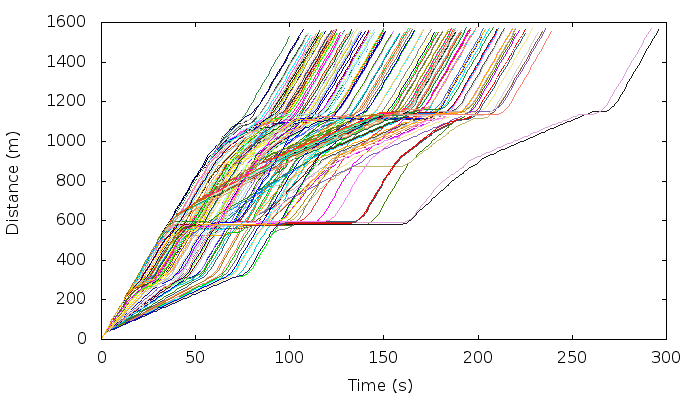
\includegraphics[width=0.45\textwidth]{../images/tp0c0_8/distanceControlled100.png}
\caption{Travel distance for simulated data when 100\% use \tech}
\label{fig:TestResults:distance100}
\end{figure}

\begin{figure}[htb]
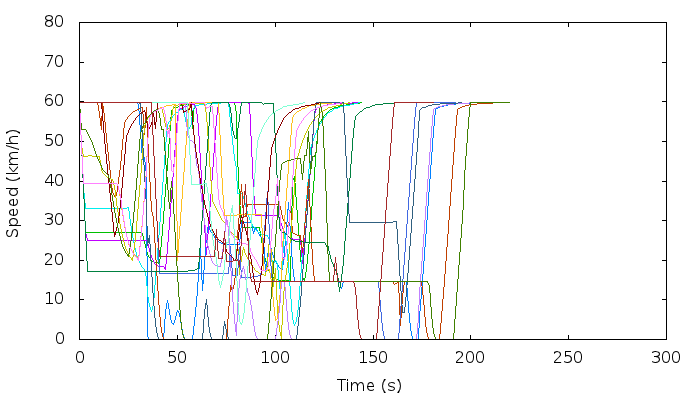
\includegraphics[width=0.45\textwidth]{../images/tp0c0_8/speedControlled100.png}
\caption{Driving speed for simulated data when 100\% use \tech}
\label{fig:TestResults:speed100}
\end{figure}

\subsection{Travel time}
Reducing the fuel consumption is important, but it cannot be at the expense of traffic flow or the vehicles travel time.
Figure~\ref{fig:TestResults:combinedTime} show the average travel time for all vehicles on all routes in the network at different levels of penetration.
With 0 \% using \tech we see an average travel time of $139$ seconds. 
Introducing the systemt to 10 \% of the vehicles reduces this by about 2 \% ($136s$). 
However, as the penetration rate increases, we travel time continues to reduce. 
This is mostly due to the fact that vehicles do not make a full stop at traffic lights, and therefore are able to start faster.
%TODO: We should compare with real data here!

\begin{figure}[htb]
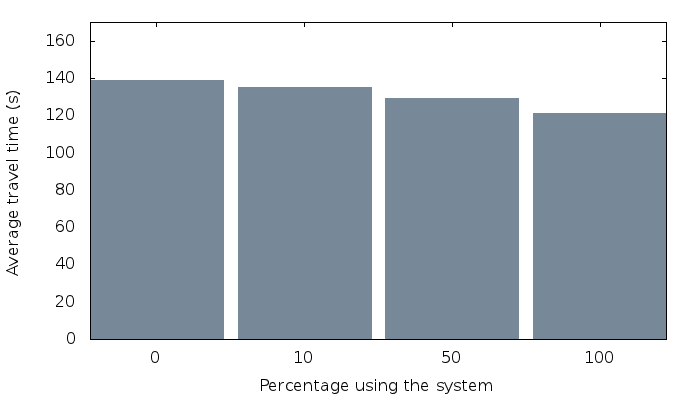
\includegraphics[width=0.45\textwidth]{../images/tp0c0_8/combinedTime.png}
\caption{Travel time for all routes at different level of vehicles using \tech}
\label{fig:TestResults:combinedTime}
\end{figure}

\subsection{Congestion levels}
%TODO: when does the traffic break? Do we break later than without \tech?
Normal traffic usualy have peak periods where the traffic is higher than normal \cite{Vejdir}. 
In order to test the effect of the system with different congestion levels we repeated the simulation while changing the rate with which vehicles are spwaning. 
The fuel consumption at different penetration rates (plots) and congestion levels (x-axis) can be seen in Figure \ref{fig:TestResults:congestionFuel}. 
The fuel consumtion does not change much when less than $1$ vehicle spawn per second.
With higher congestion, the traffic seems to break down, most pronouced at lower penetration rates. %TODO: Break down stuff
\begin{figure}[htb]
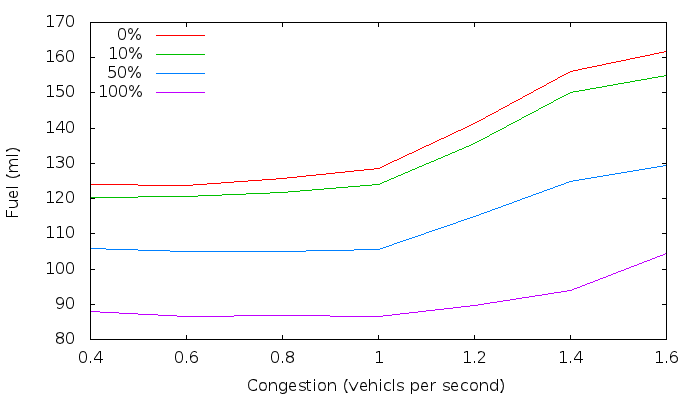
\includegraphics[width=0.45\textwidth]{../images/fuelCongestion.png}
\caption{Fuel consumption at different penetration and congestion levels}
\label{fig:TestResults:congestionFuel}
\end{figure}

In Figure \ref{fig:TestResults:congestionTime} we see the average travel time for all vehicles driving in the simulation compared to the different congestion levels. 
With low congestion there is almost no difference in the travel time.
We clearly see that the travel time increases less when more drivers use \tech as the congestion increases. %TODO: Break down stuff
In a congested network large queues of vehicles build up. 
A large portion of the time a traffic light is green is wasted on the time it takes to get the queue moving. 
A queue of vehicles accelerrating spend less time gaining speed if they are already moving slowly. 
This is likly the reason that the average time of all vehicles improve if enough are using the system.
\begin{figure}[htb]
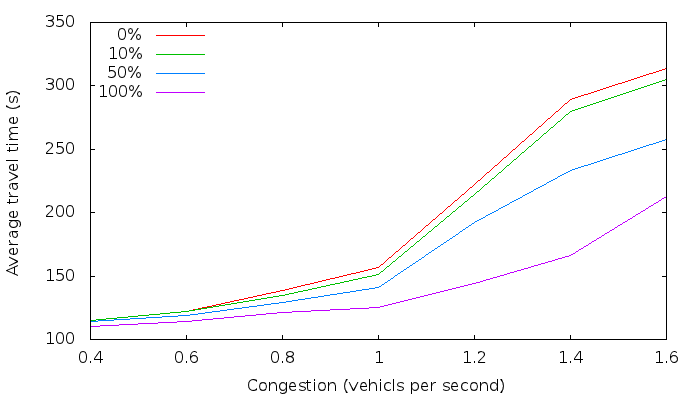
\includegraphics[width=0.45\textwidth]{../images/timeCongestion.png}
\caption{Travel time at different penetration and congestion levels}
\label{fig:TestResults:congestionTime}
\end{figure}

\section{Potential Savings}
%TODO: do this

